%%%%%%%%%%%%%%%%%%%%%%%%%%%%%%%%%%%%%%%%%
% Beamer Presentation
% LaTeX Template
% Version 1.0 (10/11/12)
%
% This template has been downloaded from:
% http://www.LaTeXTemplates.com
%
% License:
% CC BY-NC-SA 3.0 (http://creativecommons.org/licenses/by-nc-sa/3.0/)
%
%%%%%%%%%%%%%%%%%%%%%%%%%%%%%%%%%%%%%%%%%

%----------------------------------------------------------------------------------------
%	PACKAGES AND THEMES
%----------------------------------------------------------------------------------------

\documentclass[10pt]{beamer}
%\documentclass[]{beamer}
\usepackage{etex}
\mode<presentation>
%\usetheme{Warsaw}

%\useoutertheme{smoothtree}
%\useoutertheme{split}
%\useoutertheme[hideothersubsections]{sidebar}
%\useoutertheme[]{smoothbars}
%\useoutertheme[]{miniframes}
%\useoutertheme{infolines}
\addtobeamertemplate{headline}{}{\vskip2pt}


% The Beamer class comes with a number of default slide themes
% which change the colors and layouts of slides. Below this is a list
% of all the themes, uncomment each in turn to see what they look like.

%\usetheme{default}
%\usetheme{AnnArbor}
%\usetheme{Antibes}
%\usetheme{Bergen}
%\usetheme{Berkeley}
%\usetheme{Berlin}
\usetheme{Boadilla}
%\usetheme{CambridgeUS}
%\usetheme{Copenhagen}
%\usetheme{Darmstadt}
%\usetheme{Dresden}
%\usetheme{Frankfurt}
%\usetheme{Goettingen}
%\usetheme{Hannover}
%\usetheme{Ilmenau}
%\usetheme{JuanLesPins}
%\usetheme{Luebeck}
%\usetheme{Madrid}
%\usetheme{Malmoe}
%\usetheme{Marburg}
%\usetheme{Montpellier}
%\usetheme{PaloAlto}
%\usetheme{Pittsburgh}
%\usetheme{Rochester}
%\usetheme{Singapore}
%\usetheme{Szeged}


% As well as themes, the Beamer class has a number of color themes
% for any slide theme. Uncomment each of these in turn to see how it
% changes the colors of your current slide theme.

%\usecolortheme{albatross}
%\usecolortheme{beaver}
%\usecolortheme{beetle}
%\usecolortheme{crane}
%\usecolortheme{dolphin}
%\usecolortheme{dove}
%\usecolortheme{fly}
%\usecolortheme{lily}
%\usecolortheme{orchid}
%\usecolortheme{rose}
%\usecolortheme{seagull}
%\usecolortheme{seahorse}
%\usecolortheme{whale}
%\usecolortheme{wolverine}

%\setbeamertemplate{footline} % To remove the footer line in all slides uncomment this line
%\setbeamertemplate{footline}[page number] % To replace the footer line in all slides with a simple slide count uncomment this line

%\setbeamertemplate{navigation symbols}{} % To remove the navigation symbols from the bottom of all slides uncomment this line

\useinnertheme{rectangles}
\setbeamertemplate{navigation symbols}{}
\setbeamertemplate{footline}[frame number]
\setbeamertemplate{caption}[numbered]
\usepackage{amsmath,amsthm,amssymb} %math stuff
\usepackage{beamerthemesplit}
\usepackage{comment} 
\usepackage{hyperref}
\usepackage{xfrac}
\usepackage{dtklogos}
\usepackage{wrapfig}
\usepackage{subcaption}
\usepackage{ctable}
\usepackage{pdfpages}
\usepackage{xparse}
%\usepackage{verbatim}
%\hypersetup{pdfpagemode=FullScreen} % makes your presentation go automatically to full screen
\usepackage{graphicx} % Allows including images
\usepackage{booktabs} % Allows the use of \toprule, \midrule and \bottomrule in tables
\definecolor{Gray}{gray}{0.9}
\definecolor{Red}{rgb}{0.9,.6,.8}
\definecolor{LightCyan}{rgb}{0.88,1,1}
\usepackage{color, colortbl}
\newcommand{\mc}[2]{\multicolumn{#1}{c}{#2}}
\newcommand{\oddsr}[1]{\left( \dfrac{{#1}}{1-{#1}}\right)}
\setbeamercovered{highly dynamic}

\NewDocumentCommand\mylist{>{\SplitList{;}}m}
  {
    \begin{itemize}
      \ProcessList{#1}{ \insertitem }
    \end{itemize}
  }
\newcommand\insertitem[1]{\item #1}

\newcounter{saveenumi}
\newcommand{\seti}{\setcounter{saveenumi}{\value{enumi}}}
\newcommand{\conti}{\setcounter{enumi}{\value{saveenumi}}}

\resetcounteronoverlays{saveenumi}
%----------------------------------------------------------------------------------------
%	TITLE PAGE
%----------------------------------------------------------------------------------------

\title[\LaTeX Tutorial]{Introduction to \LaTeX} % The short title appears at the bottom of every slide, the full title is only on the title page

\author{Sahir Rai Bhatnagar} % Your name
\institute[Queen's University] % Your institution as it will appear on the bottom of every slide, may be shorthand to save space
{
Queen's University \\ % Your institution for the title page
\medskip
\textit{12sb32@queensu.ca} % Your email address
}
\date{\today} % Date, can be changed to a custom date

\begin{document}

\maketitle


\section{Introduction}
\subsection{What is \LaTeX ?}
\begin{frame}[fragile]\frametitle{A powerful Typesetting system}

\begin{columns}[c] % The "c" option specifies centered vertical alignment while the "t" option is used for top vertical alignment

\column{.25\textwidth} % Left column and width
{\tiny
\begin{verbatim}
A \textbf{bold 
\textit{Hello \LaTeX}} 
to start!
\end{verbatim}
}
A \textbf{bold \textit{Hello \LaTeX}} to start !

{\tiny
\begin{verbatim}
Odds=$\left(\frac{\pi}{1-\pi} 
\right)$ 
\end{verbatim}
}

Odds=$\left( \frac{\pi}{1-\pi} \right) $




\column{.7\textwidth} % Right column and width
\small
\begin{enumerate}
%\item Used for producing scientific and mathematical documents
\item Input for \LaTeX \, is composed in plain \texttt{ASCII} using a text editor
%\item Unike Word, \LaTeX\, \textbf{\textit{is not}} What you see is what you get (WYSIWYG)
\item Although Word is useful for writing very short and simple documents, it becomes too complex or even unusable for more complicated tasks
\item Commonly needed features, like user-customized automated numbering or various automated indexes, cannot be created using Word at all
\item \LaTeX \,does require more effort and time to learn to use even for simpler tasks, but once learned, difficult tasks can be accomplished rather easily and straightforwardly
\end{enumerate}

\end{columns}

\end{frame}

\begin{frame}\frametitle{What is \texttt{ASCII}?}

\begin{columns}[c] % The "c" option specifies centered vertical alignment while the "t" option is used for top vertical alignment

\column{.3\textwidth} % Left column and width
\begin{figure}[h!]
\centering
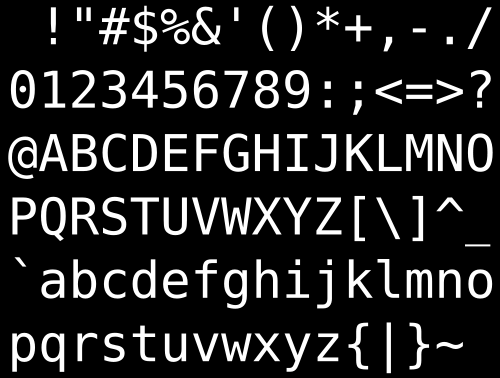
\includegraphics[scale=0.2, keepaspectratio]{./ASCIIfull}
\caption{95 printable \texttt{ASCII} characters, numbered 32 to 126. (0 to 31 \& 127 are non-printing control characters) }
\label{fig:ascii}
\end{figure}

\column{.7\textwidth} % Right column and width
\begin{enumerate}
\item When you save your document, it is saved in the form of plain text i.e in ``\texttt{ASCII}'' (the American Standard Code for Information Interchange)
\item \texttt{ASCII} is composed of 128 ($2^7$) characters: 7 binary digits for its encoding (Fig. \ref{fig:ascii})
\item An \texttt{ASCII} message will be understandable by any computer in the world. If you send such a message, you can be sure that the recipient will see precisely what you typed
\seti
\end{enumerate}
\end{columns}
\end{frame} 

\begin{frame}\frametitle{What is \texttt{ASCII}?}

\begin{enumerate}
\conti
\item By contrast, when you save a file from a word processor, the file contains various control characters, outside of the \texttt{ASCII} range. These characters represent the formatting that you applied (e.g.  boldface or italics) plus various sorts of internal ``business'' relating to the mechanics of the word processor
\item They are not universally understandable: to make sense of them, you need a copy of the word processor with which the document was created
\item If you open a word processor file in a text editor, you will see (besides the text, or bits of it) a lot of funny looking stuff: this is the binary formatting code.
\end{enumerate}

\end{frame} 

\subsection{\LaTeX \, vs. Word}
\begin{frame}\frametitle{Comparison}
\begin{columns}[c] % The "c" option specifies centered vertical alignment while the "t" option is used for top vertical alignment

\column{.45\textwidth} % Left column and width
\begin{figure}[h!]
\centering
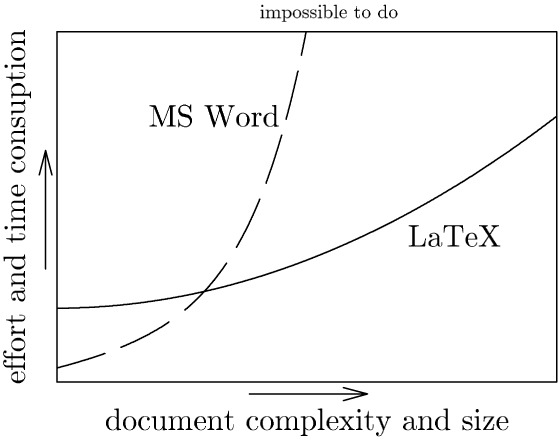
\includegraphics[scale=1, keepaspectratio]{./miktex}
\caption{Comparison}
\label{fig:word}
\end{figure}

\column{.5\textwidth} % Right column and width
\begin{itemize}
\item \LaTeX \, has a greater learning curve
\item Many tasks are very tedious or impossible (most cases) to do in MS Word or Libre Office
\end{itemize}
\end{columns}

\end{frame}


%\begin{comment}

\begin{frame}\frametitle{The Philosophy behind \LaTeX}
\begin{columns}[c] % The "c" option specifies centered vertical alignment while the "t" option is used for top vertical alignment

\column{.45\textwidth} % Left column and width
\begin{figure}[h!]
\centering
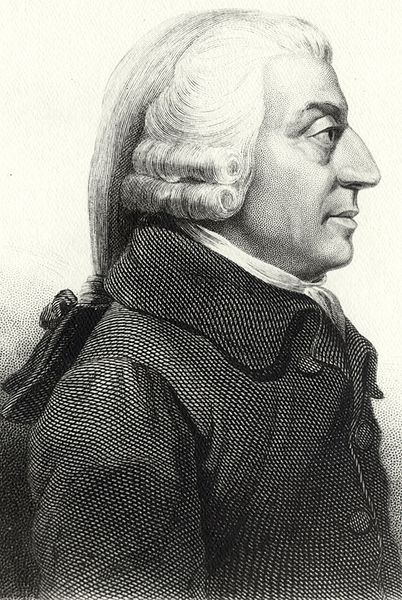
\includegraphics[scale=0.6, keepaspectratio]{./smith}
\small
\caption{Adam Smith, author of \textit{The Wealth of Nations} (1776), in which he conceptualizes the notion of the division of labour}
\label{fig:smith}
\end{figure}

\column{.5\textwidth} % Right column and width
\small
\begin{block}{Division of Labour}
Composition and logical structuring of text is the author's specific contribution to the production of a printed text. Matters such as the choice of the font family, should section headings be in bold face or small capitals? Should they be flush left or centered? Should the text be justified or not? Should the notes appear at the foot of the page or at the end? Should the text be set in one column or two? and so on, is the typesetter's business
\end{block}
\end{columns}

\end{frame}


\begin{frame}\frametitle{The Philosophy behind \LaTeX}

\begin{block}{Problems with ``What you see is what you get'' (WYSIWYG) editors such as MS Word and LibreOffice}
\begin{enumerate}
\item Author is distracted from the proper business of composing text, in favour of making typographical choices in relation to which they may have no expertise i.e. fiddling with fonts and margins when they should be concentrating on content
\item Making changes to the whole document i.e. section headings, numbering of figures, references and tables is tedious
\item Does not encourage concern with document structure
\end{enumerate}
\end{block}


\end{frame}


%\end{comment}


\subsection{Advantages}
\begin{frame}{Many Reasons to use \LaTeX}
\begin{itemize}
\item The typesetting of mathematical formulae is supported in a convenient way
\item  Users only need to learn a few easy-to-understand commands that specify the logical structure of a document. They almost never need to
tinker with the actual layout of the document
\item Even complex structures such as footnotes, references, table of contents, and bibliographies can be generated easily.
\item \LaTeX \, encourages authors to write well-structured texts, because this is how \LaTeX \, works: by specifying structure
\item \TeX, the formatting engine of \LaTeXe, is highly portable and free. Therefore the system runs on almost any hardware platform available
\end{itemize}
\end{frame}




\subsection{History}

\begin{frame}\frametitle{The Genius Behind \LaTeX}
\small
The \TeX \,project was started in 1978 by Don­ald E. Knuth (University of Stanford), while re­vis­ing the sec­ond vol­ume of his \textit{Art of Com­puter Pro­gramming}. He saw that the pub­lisher had switched to a new dig­i­tal type­set­ting sys­tem and was shocked at the poor qual­ity.
\begin{wrapfigure}{r}{0.5\textwidth}
  \vspace{-20pt}
  \begin{center}
    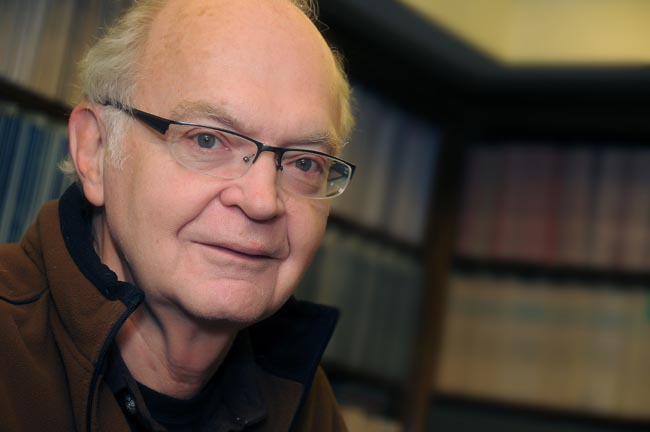
\includegraphics[scale=0.2, keepaspectratio]{./don}
  \end{center}
  \vspace{-20pt}
  \caption{Donald E. Knuth}
  \vspace{-10pt}
\end{wrapfigure}
He rea­soned that be­cause dig­i­tal type­set­ting meant ar­rang­ing 1's and 0's in the proper pat­tern, as a com­puter sci­en­tist he should be able to do the job bet­ter. He orig­i­nally es­ti­mated that this would take six months but ul­ti­mately it took nearly ten years. He had to han­dle not only the chal­lenges of rou­tine type­set­ting such as right-jus­ti­fi­ca­tion and page for­mat­ting flex­i­ble enough to al­low for dif­fer­ent out­put styles, but also the ad­di­tional de­mands of aca­demic pub­lish­ing – foot­notes, float­ing fig­ures and ta­bles, etc. And, be­yond that, he had to tell the com­puter how to type­set for­mu­las and other tech­ni­cal ma­te­ri­als.

\end{frame}

\section{References}
\begin{frame}[allowframebreaks]
\frametitle<presentation>{References}    
\bibliographystyle{amsalpha}
\nocite{allin}
\nocite{ctan}
\nocite{latexdocs}
\nocite{pinteric}
\nocite{lamport}
\nocite{short}
\nocite{ams}
\nocite{gentle}
\nocite{ams}
\nocite{online}
\nocite{spellcheck}
\bibliography{tutorial.bib}
\end{frame}


\end{document}